%% This is the main file and you use this file to organize your assignment.

\documentclass[a4paper]{article}
\usepackage[margin=3cm]{geometry} 	   % Choose your margin here.
\usepackage{amsmath}
\usepackage{parskip}
\usepackage{graphicx}
\usepackage{caption}
\usepackage{subcaption}
\usepackage{listings}
\usepackage{color} %red, green, blue, yellow, cyan, magenta, black, white
\definecolor{mygreen}{RGB}{28,172,0} % color values Red, Green, Blue
\definecolor{mylilas}{RGB}{170,55,241}

\newcommand{\figref}[1]{\figurename~\ref{#1}}
\renewcommand\thesection{Problem \arabic{section}}
\renewcommand\thesubsection{Problem \arabic{section}.\arabic{subsection}}

\let\endtitlepage\relax						% Begin the text immidiately after the title page. Optional
\setlength{\parindent}{0cm}				% Start paragraph without indent. Optional

\begin{document}

\lstset{language=Matlab,%
    breaklines=true,%
    morekeywords={matlab2tikz},
    keywordstyle=\color{blue},%
    morekeywords=[2]{1}, keywordstyle=[2]{\color{black}},
    identifierstyle=\color{black},%
    stringstyle=\color{mylilas},
    commentstyle=\color{mygreen},%
    showstringspaces=false,%without this there will be a symbol in the places where there is a space
    numbers=left,%
    numberstyle={\tiny \color{black}},% size of the numbers
    numbersep=9pt, % this defines how far the numbers are from the text
    emph=[1]{for, end, break}\emphstyle=[1]\color{red}, %some words to emphasise
}

\begin{titlepage}
\begin{center}
\Large TTK4190 Guidance and Control of Vehicles \\
\vspace{10pt}
\Large Assignment 1 \\
\vspace{10pt}
\large Written Fall 2019 By Sigurd Totland
\end{center}
\end{titlepage}

\section*{Info}
This is only a short template for the assignments and it is definitely not necessary to use this template if you are familiar with \LaTeX{} beforehand. The best way to learn \LaTeX{} is to write some stuff yourself and Google problems you run into. Therefore, we will not answer \LaTeX{} related questions outside of the assignment guidance, but you are of course welcome to ask questions then.

\section*{Problem 1 - Attitude Control of Satellite}
You can answer Problem 1 in this file/section. One subsection for each part of the problem might be a good solution. 

\subsection*{Problem 1.1} 
This is where you answer Problem 1.1. Equation (1) from the assignment can be written in \LaTeX{} as:
\begin{equation}
\label{eq:dynamics}		% The label is used when referring to this equation. 
	\begin{aligned}
		\dot{\mathbf{q}} = \mathbf{T}_q (\mathbf{q} ) \boldsymbol{\omega} \\
		\mathbf{I}_{CG} \dot{\boldsymbol{\omega}} - \mathbf{S} (\mathbf{I}_{CG} \boldsymbol{\omega} ) \boldsymbol{\omega} & =  \boldsymbol{\tau}
	\end{aligned}	
\end{equation}
You can now refer to this equation as \eqref{eq:dynamics} where the label ensures that the correct equation number is used. If you want to write an equation directly in the text (outside of the equation environment), use: $\dot{\mathbf{q}} = \mathbf{T}_q (\mathbf{q} ) \boldsymbol{\omega}$. % You have to use the dollar sign to write math symbols within a text. 

A matrix (and an equation without equation number) can be created as: 
\begin{equation*}	% The star indicates that you don't want to give this equation a number. Normally used if you don't refer to the equation.
	\mathbf{A} = 
	\begin{bmatrix}
		a & b & c \\ d & e & f \\ g & h & i
	\end{bmatrix} \quad
	\mathbf{B} = 
	\begin{bmatrix}
		a \\ b \\ c
	\end{bmatrix}
\end{equation*}

\subsection*{Problem 1.2}
Answer Problem 1.2 here. Bold words can be written as \textbf{something bold}. It is also possible to create a new section level:
\subsubsection*{Inner Section 1}
\emph{text..}

\subsubsection*{Inner Section 2}
...

\subsection*{Problem 1.3}
Answer Problem 1.3 here. Equation (2) from the assignment can be written as: 
\begin{equation}
  \label{eq:tau}
  \mathbf{\tau} = -\mathbf{K}_d \boldsymbol{\omega} - k_p \boldsymbol{\epsilon}
\end{equation}

\subsection*{Problem 1.4}
The quaternion error can be written as
 \begin{equation}
	 \tilde{\mathbf{q}} := \left[
	 \begin{array}{c}
		 \tilde{\eta} \\
		 \tilde{\epsilon}
	 \end{array}
	 \right] = \bar{\mathbf{q}}_d \otimes \mathbf{q} 
 \end{equation}

\subsection*{Problem 1.5}
In problems with simulations, you need to include figures in the report:
\begin{figure}[ht]
	\centering
	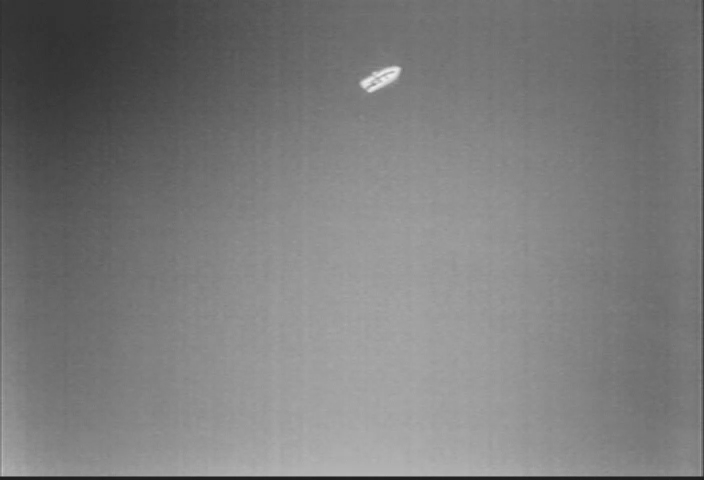
\includegraphics[width=0.7\textwidth]{fig1} % Filename is "fig1.png" and must be located in the same folder as this file. If you have a folder containing all the figures you can use "Figures/fig 1" as long as the "Figures" folder is placed in the same folder as this file.
	\caption{Figure of something useful.}
	\label{fig:fig1}
\end{figure}

You can now refer to this figure as \figref{fig:fig1}. You can also insert figures side-by-side as in Figure \ref{fig:2}. %Notice that \figref includes the word Figure before the reference. If you use "\ref", you need to write the word Figure yourself. 
\begin{figure}[ht]
	\centering
	\begin{subfigure}[b]{0.45\textwidth}
		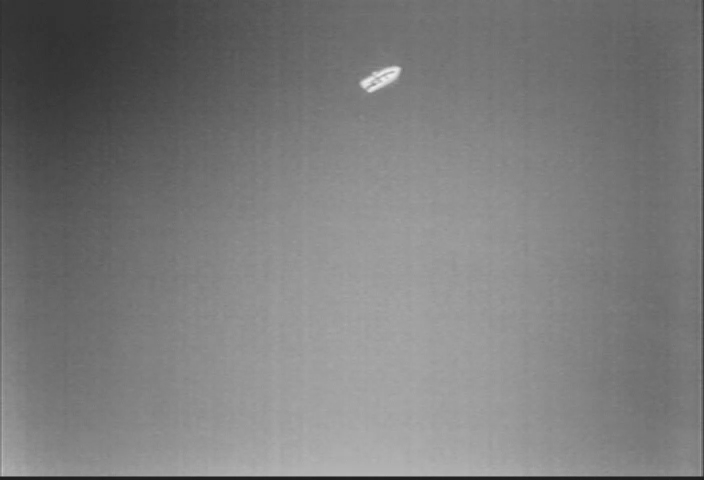
\includegraphics[width=\textwidth]{fig1}
		\caption{caption..}
		\label{fig:2a}
	\end{subfigure}
	~ %add desired spacing between images, e. g. ~, \quad, \qquad, \hfill etc. 
	%(or a blank line to force the subfigure onto a new line)
	\begin{subfigure}[b]{0.45\textwidth}
		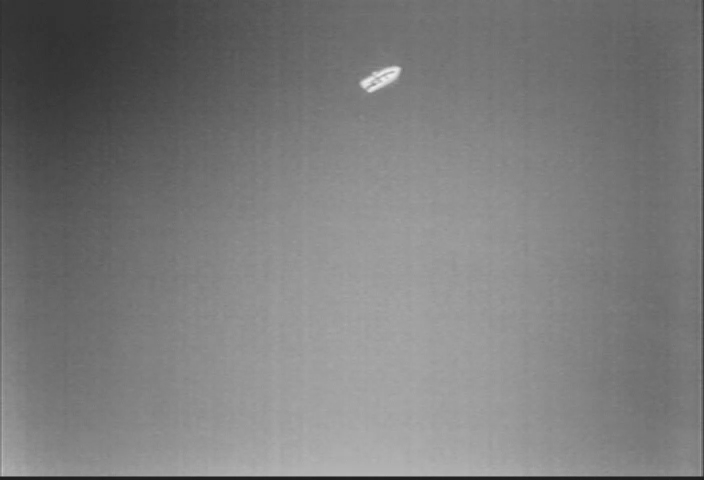
\includegraphics[width=\textwidth]{fig1}
		\caption{caption..}
		\label{fig:2b}
	\end{subfigure}
	\begin{subfigure}[b]{0.45\textwidth}
		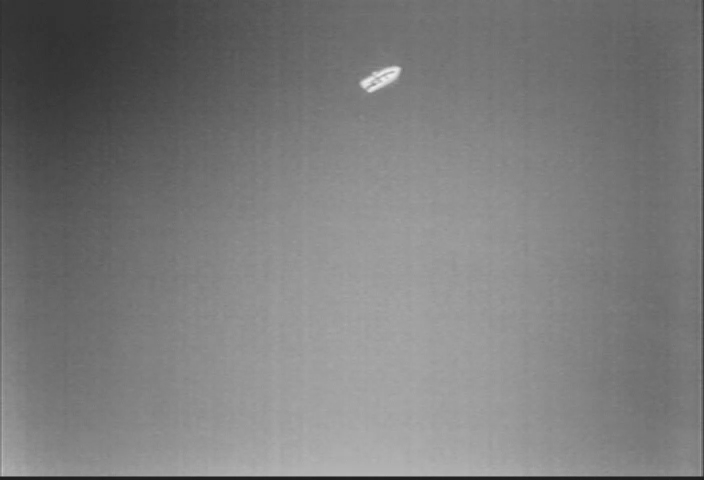
\includegraphics[width=\textwidth]{fig1}
		\caption{caption..}
		\label{fig:2c}
	\end{subfigure}
	\begin{subfigure}[b]{0.45\textwidth}
		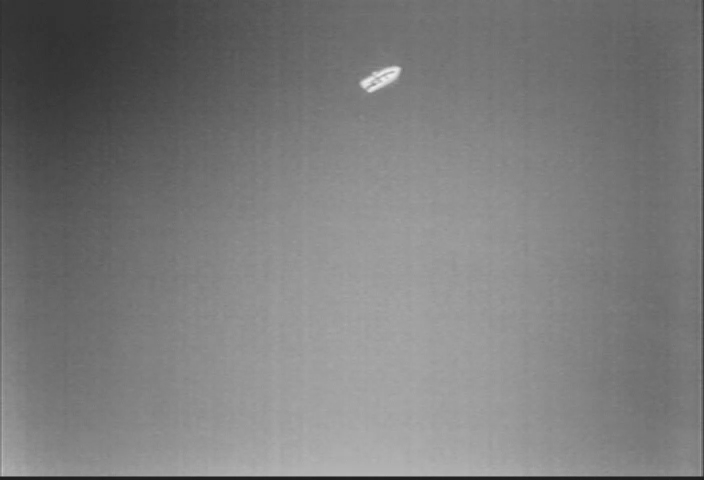
\includegraphics[width=\textwidth]{fig1}
		\caption{caption..}
		\label{fig:2d}
	\end{subfigure}		
	\caption{Caption for all figures}\label{fig:2}
\end{figure}


\subsection*{Problem 1.6}
The control law in this problem can be written as
\begin{equation}
	\boldsymbol{\tau} = -\mathbf{K}_d \tilde{\boldsymbol{\omega}} - k_p \tilde{\boldsymbol{\epsilon}}
\end{equation}
and the desired angular velocity as
\begin{equation}
	\boldsymbol{\omega}_d = \mathbf{T}^{-1}_{\Theta_d}(\Theta_d)\dot{\Theta}_d
\end{equation}

\subsection*{Problem 1.7}
The Lyapunov function can be written as 
 \begin{equation}
	 V = \frac{1}{2} \tilde{\boldsymbol{\omega}}^{\top} \mathbf{I}_{CG}\tilde{\boldsymbol{\omega}} + 2 k_p (1-\tilde{\eta})
 \end{equation}
and the derivative as 
\begin{equation}
	\dot{V} = -k_d \boldsymbol{\omega}^{\top} \boldsymbol{\omega}
\end{equation}

% Note that \mathbf can be used for bold letters in math mode (within equations and dollar signs). \boldsymbol can be used to get bold greek letters.  	% Use "\include" instead of "\input" if you want the section to start on a new page. "problem1" is a tex file included at this location in the document. It is possible to answer the whole assignment in the main file (paste everything from "problem1.tex" and "problem2.tex" here), but that restricts the readability. Therefore, one file is created for each problem.
\section{Straight-line path following in the horizontal plane}
\subsection{}
From (2.25) we have: 
\begin{equation}
	\dot{\mathbf{p}}^b_{nb} = \mathbf{R}(\mathbf{\Theta_{nb}}) \mathbf{v}^b_{nb}
\end{equation}

Then: 
\begin{align*}
	\dot{x} &= u \cos(\psi) \cos (\theta) + v [\cos (\psi) \sin( \theta) \sin (\phi) - \sin (\psi) \cos (\theta)] \\
	&+ w [\sin (\psi) \sin (\phi) + \cos (\psi) \cos (\phi) \sin(\theta)] \\
	&= u \cos(\psi) * 1 + v [\cos (\psi) * 0 * 0 - \sin (\psi) * 1] + w [\sin (\psi) * 0 + \cos (\psi) * 1 * 0] \\
	&= u \cos(\psi) - v \sin(\psi) \\
	\dot{y} &= u \sin (\psi) \cos (\theta) 
	+ v [\cos (\psi) \cos (\phi) + \sin (\phi) \sin (\theta) \sin (\psi)] \\
	&+ w [\sin (\theta) \sin (\psi) \cos (\phi) + \cos(\psi) \sin(\phi)] \\ 
	&= u \sin (\psi) * 1
	+ v [\cos (\psi) * 1 + \sin (\phi) * 0 * 0] 
	+ w [0 * \sin (\psi) * 1 + \cos(\psi) * 0] \\ 
	&= u \sin (\psi) + v \cos (\psi) 
\end{align*}
Using: 
\begin{align}
	\sin (\arctan (x)) &= \frac{x}{1 + x^2} \\
	\cos (\arctan (x)) &= \frac{1}{1 + x^2} \\ 
	U &= \sqrt{u^2 + v^2} \\ 
	\beta &= \arctan(\frac{v}{u}) \\
	\chi &= \psi + \beta 
\end{align}

We have: 
\begin{align*}
	\dot{x} &= u \cos(\psi) - v \sin(\psi) 
	= \sqrt{u^2 + v^2} [\cos (\psi) \frac{u}{\sqrt{u^2 + v^2}} 
	- \sin (\psi) \frac{v}{\sqrt{u^2 + v^2}}] \\
	&= U [\cos (\psi) \frac{1}{\sqrt{1 + \frac{v^2}{u^2}}} 
	- \sin (\psi) \frac{\frac{v}{u}}{\sqrt{1 + \frac{v^2}{u^2}}}] \\ 
	&= U [\cos (\psi) \cos(\arctan(\frac{v}{u})) 
	- \sin (\psi) \sin(\arctan(\frac{v}{u}))] 
	= U [\cos (\psi) \cos(\beta)) - \sin (\psi) \sin(\beta))] \\ 
	&= U \cos(\psi + \beta) = U \cos(\chi) \\
	\dot{y} &= u \sin (\psi) + v \cos (\psi) 
	= \sqrt{u^2 + v^2} [\sin (\psi) \frac{u}{\sqrt{u^2 + v^2}}
	+ \cos (\psi) \frac{v}{\sqrt{u^2 + v^2}}] \\
	&= U [\sin (\psi) \frac{1}{\sqrt{1 + \frac{v^2}{u^2}}} 
	+ \cos (\psi) \frac{\frac{v}{u}}{\sqrt{1 + \frac{v^2}{u^2}}}] 
	= U [\sin (\psi) \cos (\arctan(\frac{v}{u}))
	+ \cos (\psi) \sin (\arctan(\frac{v}{u}))] \\
	&= U \sin(\psi + \arctan (\frac{v}{u})) 
	= U \sin(\psi + \beta) 
	= U \sin(\chi)
\end{align*}

Answer problem 2.1 here. The Greek letters for sideslip, heading and course are $\beta$, $\psi$ and $\chi$, respectively. Equation (10) in the assignment is:
\begin{equation}
\label{y_kinematics}
	\begin{aligned}
		\dot{x} &= u \cos (\psi) -v \sin (\psi) \\
		\dot{y} &= u \sin (\psi) + v \cos (\psi)
	\end{aligned}
\end{equation}
You can refer to equations in the report by using the label and the "eqref" command. Example: equation \eqref{y_kinematics} shows the north and east velocities.

\subsection{}
Answer Problem 2.2 here...

\subsection{}
Transfer functions can be written as
\begin{equation}
	H(s) = \frac{a_n s^n + ... + a_1 s + a_0}{b_m s^m + ... + b_1 s + b_0}
\end{equation}

The Nomoto model can be written as
\begin{equation}
\label{eq:nomoto}
	\begin{aligned}
		T \dot{r} + r &= K \delta + b \\
		\dot{\psi} &= r
	\end{aligned}
\end{equation}

\subsection{}
Answer Problem 2.4 here.  References can be placed in the "bibliography.bib" and referred to as \cite{Fossen2011} and \cite{Fjellstad1994857}. The PID-controller is
\begin{equation}
	\delta = -k_p y - k_d \dot{y} - k_i \int y
\end{equation}


\bibliographystyle{IEEEtran}
\bibliography{bibliography.bib}

\end{document}
